\documentclass[10pt, a4paper]{article} 
\usepackage[
a4paper,
left=2cm,      
right=2cm,     
top=3cm,     
bottom=3cm,    
headheight=4em 
]{geometry}
\usepackage[utf8]{inputenc}
\usepackage{amsmath,amsthm,amssymb,xfrac}
\usepackage{fancyhdr}
\usepackage[hungarian]{babel}
\usepackage{graphicx}
\usepackage{float}
\usepackage{comment}
\usepackage{natbib}
\usepackage{empheq}
\usepackage{wrapfig}
\usepackage{chngcntr}
\usepackage{physics}
\usepackage{mathtools}
\counterwithin{figure}{section}
\usepackage{titlesec}
\usepackage{dsfont}
\usepackage{pdfpages}
\usepackage{t1enc}
\usepackage{tabto}
\usepackage{pgfplots}
\graphicspath{ {./images/} }
\setlength{\marginparwidth}{0pt}
\setlength{\marginparsep}{0pt}

\pagestyle{fancy}
\fancyhf{}
\cfoot{\thepage. oldal}
\lhead{
	\textbf{Gépelemek 1. Házi feladat}
	\\Kindlik Dániel
	\\AHU27Z
}

\newcommand{\knm}{\;\mathrm{\left[kNm\right]}}
\newcommand{\kn}{\;\mathrm{\left[kN\right]}}
\newcommand{\meter}{\mathrm{\left[m\right]}}
\newcommand{\pknm}{\mathrm{\left[kN/m\right]}}
\newcommand{\baar}{\mathrm{\left[bar\right]}}
\newcommand{\mpa}{\mathrm{\left[MPa\right]}}
\newcommand{\mm}{\mathrm{\left[mm\right]}}

\renewcommand*\contentsname{Tartalomjegyzék}
\begin{document}
	\begin{titlepage}
		\centering
		
\includegraphics[width=175pt]{ BMElogo.png } \\
		\vspace*{2cm}
		{\Huge \bfseries Karimás csőkötés tervezése} \\
		\vspace{0.5cm}
		{\Large Gépelemek mechatronikai mérnököknek 1. Házi feladat} \\
		\vspace{0.5cm}
		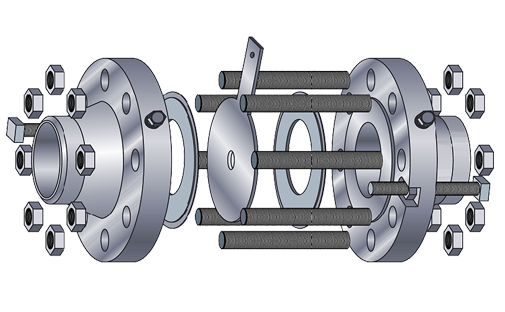
\includegraphics[width=300pt, angle=-90]{ karima_rajz.png } \\
		\vspace{1cm}
		{\Large \scshape Kindlik Dániel} \\
		\vspace{0.5cm}
		AHU27Z \\
		\vfill
		{\large \today} \\
	\end{titlepage}
	\thispagestyle{empty}
	\tableofcontents
	\newpage
	\setcounter{page}{3}
	\section*{Bevezetés}
	A feladat a megadott adatokkal egy csővéget vakkarimával lezáró csavarkötés tervezése és az elemek szilárdságilag
	ellenőrzése.
	\section{Előtervek}
	\subsection{Karima szabvány választása}
	A megadott adatok alapján ($p_{\ddot{u}} = 35\baar\;\;D_N = 32\mm$) DIN EN 1092-1 PN40 szabványt lett kiválasztva.
	\begin{figure}[h]
		\centering
		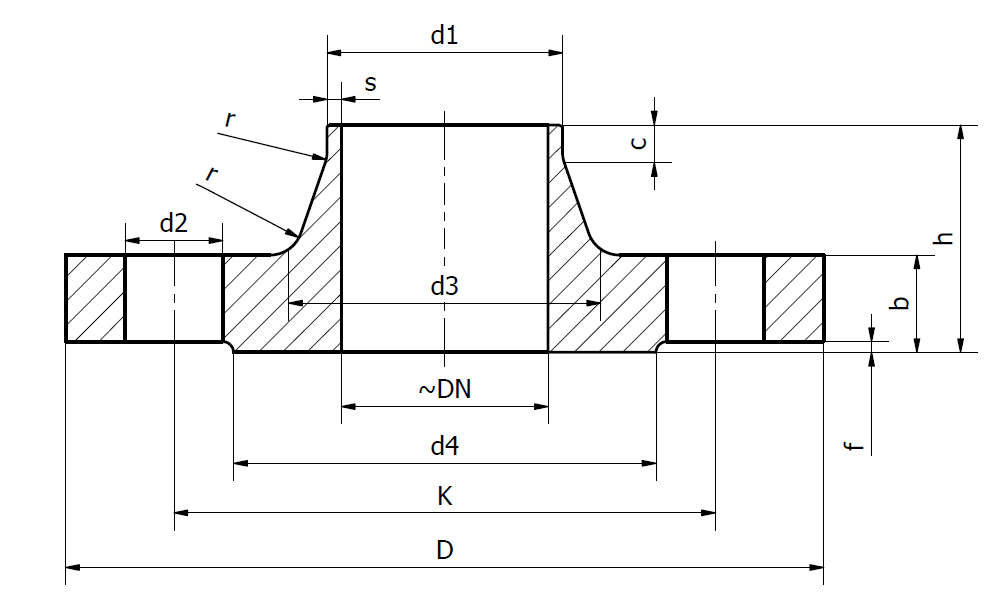
\includegraphics[width=0.75\textwidth]{ karima_eloterv.png }
		\caption{Karima előterve}
		\label{fig:karima}
	\end{figure}
	\renewcommand{\arraystretch}{1.4}
	\begin{table}[h]
		\centering
		\begin{tabular}{l|c|c}
			\textbf{Név}                              & \textbf{Jelölés} & \textbf{Érték} \\ \hline
			Karima külső átmérője                     & $D$ & 140 mm \\ 
			Karima magassága                          & $h$ & 42 mm \\ 
			Falvastagság                              & $s$ & 2.6 mm \\ 
			Kiugrás mérete                            & $f$ & 2 mm \\ 
			Kúp feletti rész magassága                & $c$                & 6 mm \\ 
			Lekerekítések nagysága                    & $r$                & 6 mm \\ 
			Cső csatlakozás külső mérete              & $d_1$             & 43.5 mm \\ 
			Csavar lyukkör átmérője                   & $d_2$             & 18 mm \\ 
			Kúp alsó átmérője                         & $d_3$             & 56 mm \\ 
			Tömítő felület külső átmérője             & $d_4$             & 78 mm \\ 
			Csavarok száma                            & $N$                & 4 db \\ 
			Csavarok mérete                           & $M$                & M16 \\ 
			Csavarok közép átmérője                   & $K$                & 100 mm \\ 
			Csavarok alapja és tömítési sík távolsága & $b$                & 18 mm \\ 
		\end{tabular}
	\end{table}
	\renewcommand{\arraystretch}{1}
	\subsection{Vakkarima szabvány választása}
	A megadott adatok alapján ($p_{\ddot{u}} = 35\baar\;\;D_N = 32\mm$) DIN EN 1092-1 PN40 szabványt lett kiválasztva.
	\begin{figure}[h]
		\centering
		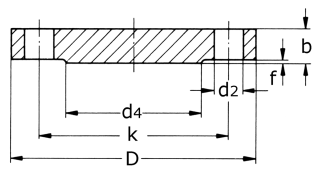
\includegraphics[width=0.5\textwidth]{ vakkarima_eloterv.png }
		\caption{Vakkarima előterve}
		\label{fig:vakkarima}
	\end{figure}
	\renewcommand{\arraystretch}{1.4}
	\begin{table}[h]
		\centering
		\begin{tabular}{l|c|c}
			\textbf{Név}                              & \textbf{Jelölés} & \textbf{Érték} \\ \hline
			Vakkarima külső átmérője                     & $D$                & 140 mm           \\
			Vakkarima magassága                          & $b$                & 18 mm			\\
			Kiugrás mérete                            & $f$                & 2 mm           \\
			Csavar lyukkör átmérője                   & $d_2$             & 18 mm           \\
			Tömítő felület külső átmérője             & $d_4$             & 78 mm           \\
			Csavarok száma                            & $N$                & 4 db           \\
			Csavarok mérete                           & $M$                & M16          \\ 
			Csavarok közép átmérője                   & $K$                & 100 mm             
		\end{tabular}
	\end{table}
	\renewcommand{\arraystretch}{1}
	\subsection{Konstrukció előterve}
	x
	\section{Vakkarima minimális vastagságának számítása, megfelelő lemezvastagság választása}
	A vakkarima minimális vastagságának kiszámításához használhatjuk az alábbi egyenletet:\\
	\begin{equation}
		b_{\text{min}} = \sqrt{\dfrac{3 \cdot p_\text{ü}}{\sigma_{\text{hajl}}} \cdot \left(1 - \dfrac{2 \cdot d_t}{3 \cdot k}\right)} \cdot \dfrac{d_t}{2}
	\end{equation}
	\renewcommand{\arraystretch}{1.4}
		\begin{table}[h]
			\centering
			\begin{tabular}{l|c|c}
				\textbf{Név}                              & \textbf{Jelölés} & \textbf{Érték} \\ \hline
				Tömítés külső átmérője                     & $p_\text{ü}$                & 78 mm           \\
				Tömítés belső átmérője                     & $\sigma_{\text{hajl}}$                & 32 mm			\\
				Tömítés vastagsága                         & $k$                & 3 mm     \\
				Tömítés vastagsága                         & $d_t$                & 3 mm           
			\end{tabular}
		\end{table}
		\renewcommand{\arraystretch}{1}	
	\section{Megfelelő lapos tömítés választása, minimális tömítési erő számítása}
	A megadott adatok alapján ($p_{\ddot{u}} = 35\baar\;\;D_N = 32\mm$) DIN EN 1092-1 DN32 SBR tömítés lett választva, ami 40 bar nyomásig használható, így PN40-es karimákhoz jó.
	\begin{figure}[h]
		\centering
		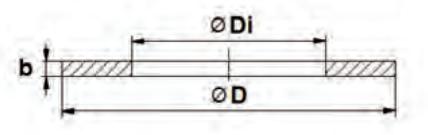
\includegraphics[width=0.5\textwidth]{ tomites_eloterv.png }
		\caption{Tömítés előterve}
		\label{fig:tomites}
	\end{figure}
	\renewcommand{\arraystretch}{1.4}
	\begin{table}[h]
		\centering
		\begin{tabular}{l|c|c}
			\textbf{Név}                              & \textbf{Jelölés} & \textbf{Érték} \\ \hline
			Tömítés külső átmérője                     & $D$                & 78 mm           \\
			Tömítés belső átmérője                     & $D_i$                & 32 mm			\\
			Tömítés vastagsága                         & $b$                & 3 mm             
		\end{tabular}
	\end{table}
	\renewcommand{\arraystretch}{1}	
	\section{Csavarra jutó terhelés számítása}
	\section{Csavar előfeszítésének és szükséges meghúzási nyomaték számítása}
	\section{Csavar anyagának kiválasztása, benne ébredő egyenfeszültség kiválasztása}
	\section{Konstrukció összeállítási rajza}
\end{document}